
\documentclass[12pt,a4paper]{article}

\usepackage[a4paper,margin=1in]{geometry}
\usepackage{graphicx}
\usepackage{booktabs}
\usepackage{amsmath,amssymb}
\usepackage{float}
\usepackage{hyperref}
\usepackage{xcolor}
\usepackage{listings}
\usepackage{enumitem}
\usepackage{fancyhdr}
\usepackage{longtable}

\hypersetup{colorlinks=true,linkcolor=blue,urlcolor=blue}

\pagestyle{fancy}
\fancyhf{}
\lhead{ICS1512}
\rhead{Machine Learning Algorithms Laboratory}
\cfoot{\thepage}

\lstset{
language=Python,
basicstyle=\ttfamily\small,
numbers=left,
frame=single,
breaklines=true,
showstringspaces=false
}

\begin{document}

\begin{tabular}{|p{4cm}|p{11cm}|}
\hline
Experiment No. & 3 \\ \hline
Experiment Title & Regression Analysis using Linear and Regularized Models\footnotemark \\ \hline
Student Name & Sanjay S \\ \hline
Register Number & 3122247001056 \\ \hline
Faculty & Dr. Poreddy Ajay Kumar Reddy \\ \hline
Submission Date & 03/08/2026 \\ \hline
\end{tabular}
\footnotetext{\textbf{GitHub Repository: }\url{https://github.com/sanjay-6727/Introdution-to-Machine-Learning-}}

\section{Objective}
Implement Linear, Ridge, Lasso and Elastic Net regression, compare all four across several error
metrics, and actually see what overfitting, underfitting and the bias-variance tradeoff look like on a
real, messy dataset instead of a textbook toy example.

\section{Problem Statement}
Given loan application records with a mix of numeric and categorical fields, predict the loan sanction
amount in USD, and figure out how much regularization is really buying you once a plain baseline linear
model is already sitting there.

\section{Dataset Description}
\begin{longtable}{|p{6cm}|p{8cm}|}
\hline
Dataset Name & Predict Loan Amount Data \\ \hline
Dataset Source & Kaggle, phileinsophos/predict-loan-amount-data \\ \hline
Number of Samples & 29322 (after removing rows with a missing or sentinel target) \\ \hline
Number of Features & 45 after one-hot encoding 9 categorical columns \\ \hline
Number of Classes & not applicable, regression target \\ \hline
Missing Values & worst columns were Type of Employment (about 24 percent), Property Age (about 16
percent), Income (about 15 percent) \\ \hline
Train-Test Split & 80/20, plus 5 fold cross validation for tuning \\ \hline
\end{longtable}

338 rows had the target sitting at $-999$, clearly just a placeholder, and another 340 rows had no
target at all. Both got dropped outright rather than imputed, since guessing the very thing you are
trying to predict felt like cheating.

\section{Exploratory Data Analysis}
\begin{itemize}
\item Target distribution: heavily right skewed, with a large spike near zero.
\item Feature vs target scatter for the four numeric fields I expected to matter most going in.
\item Correlation and missing value heatmaps across the raw numeric columns.
\end{itemize}

\begin{figure}[H]
\centering
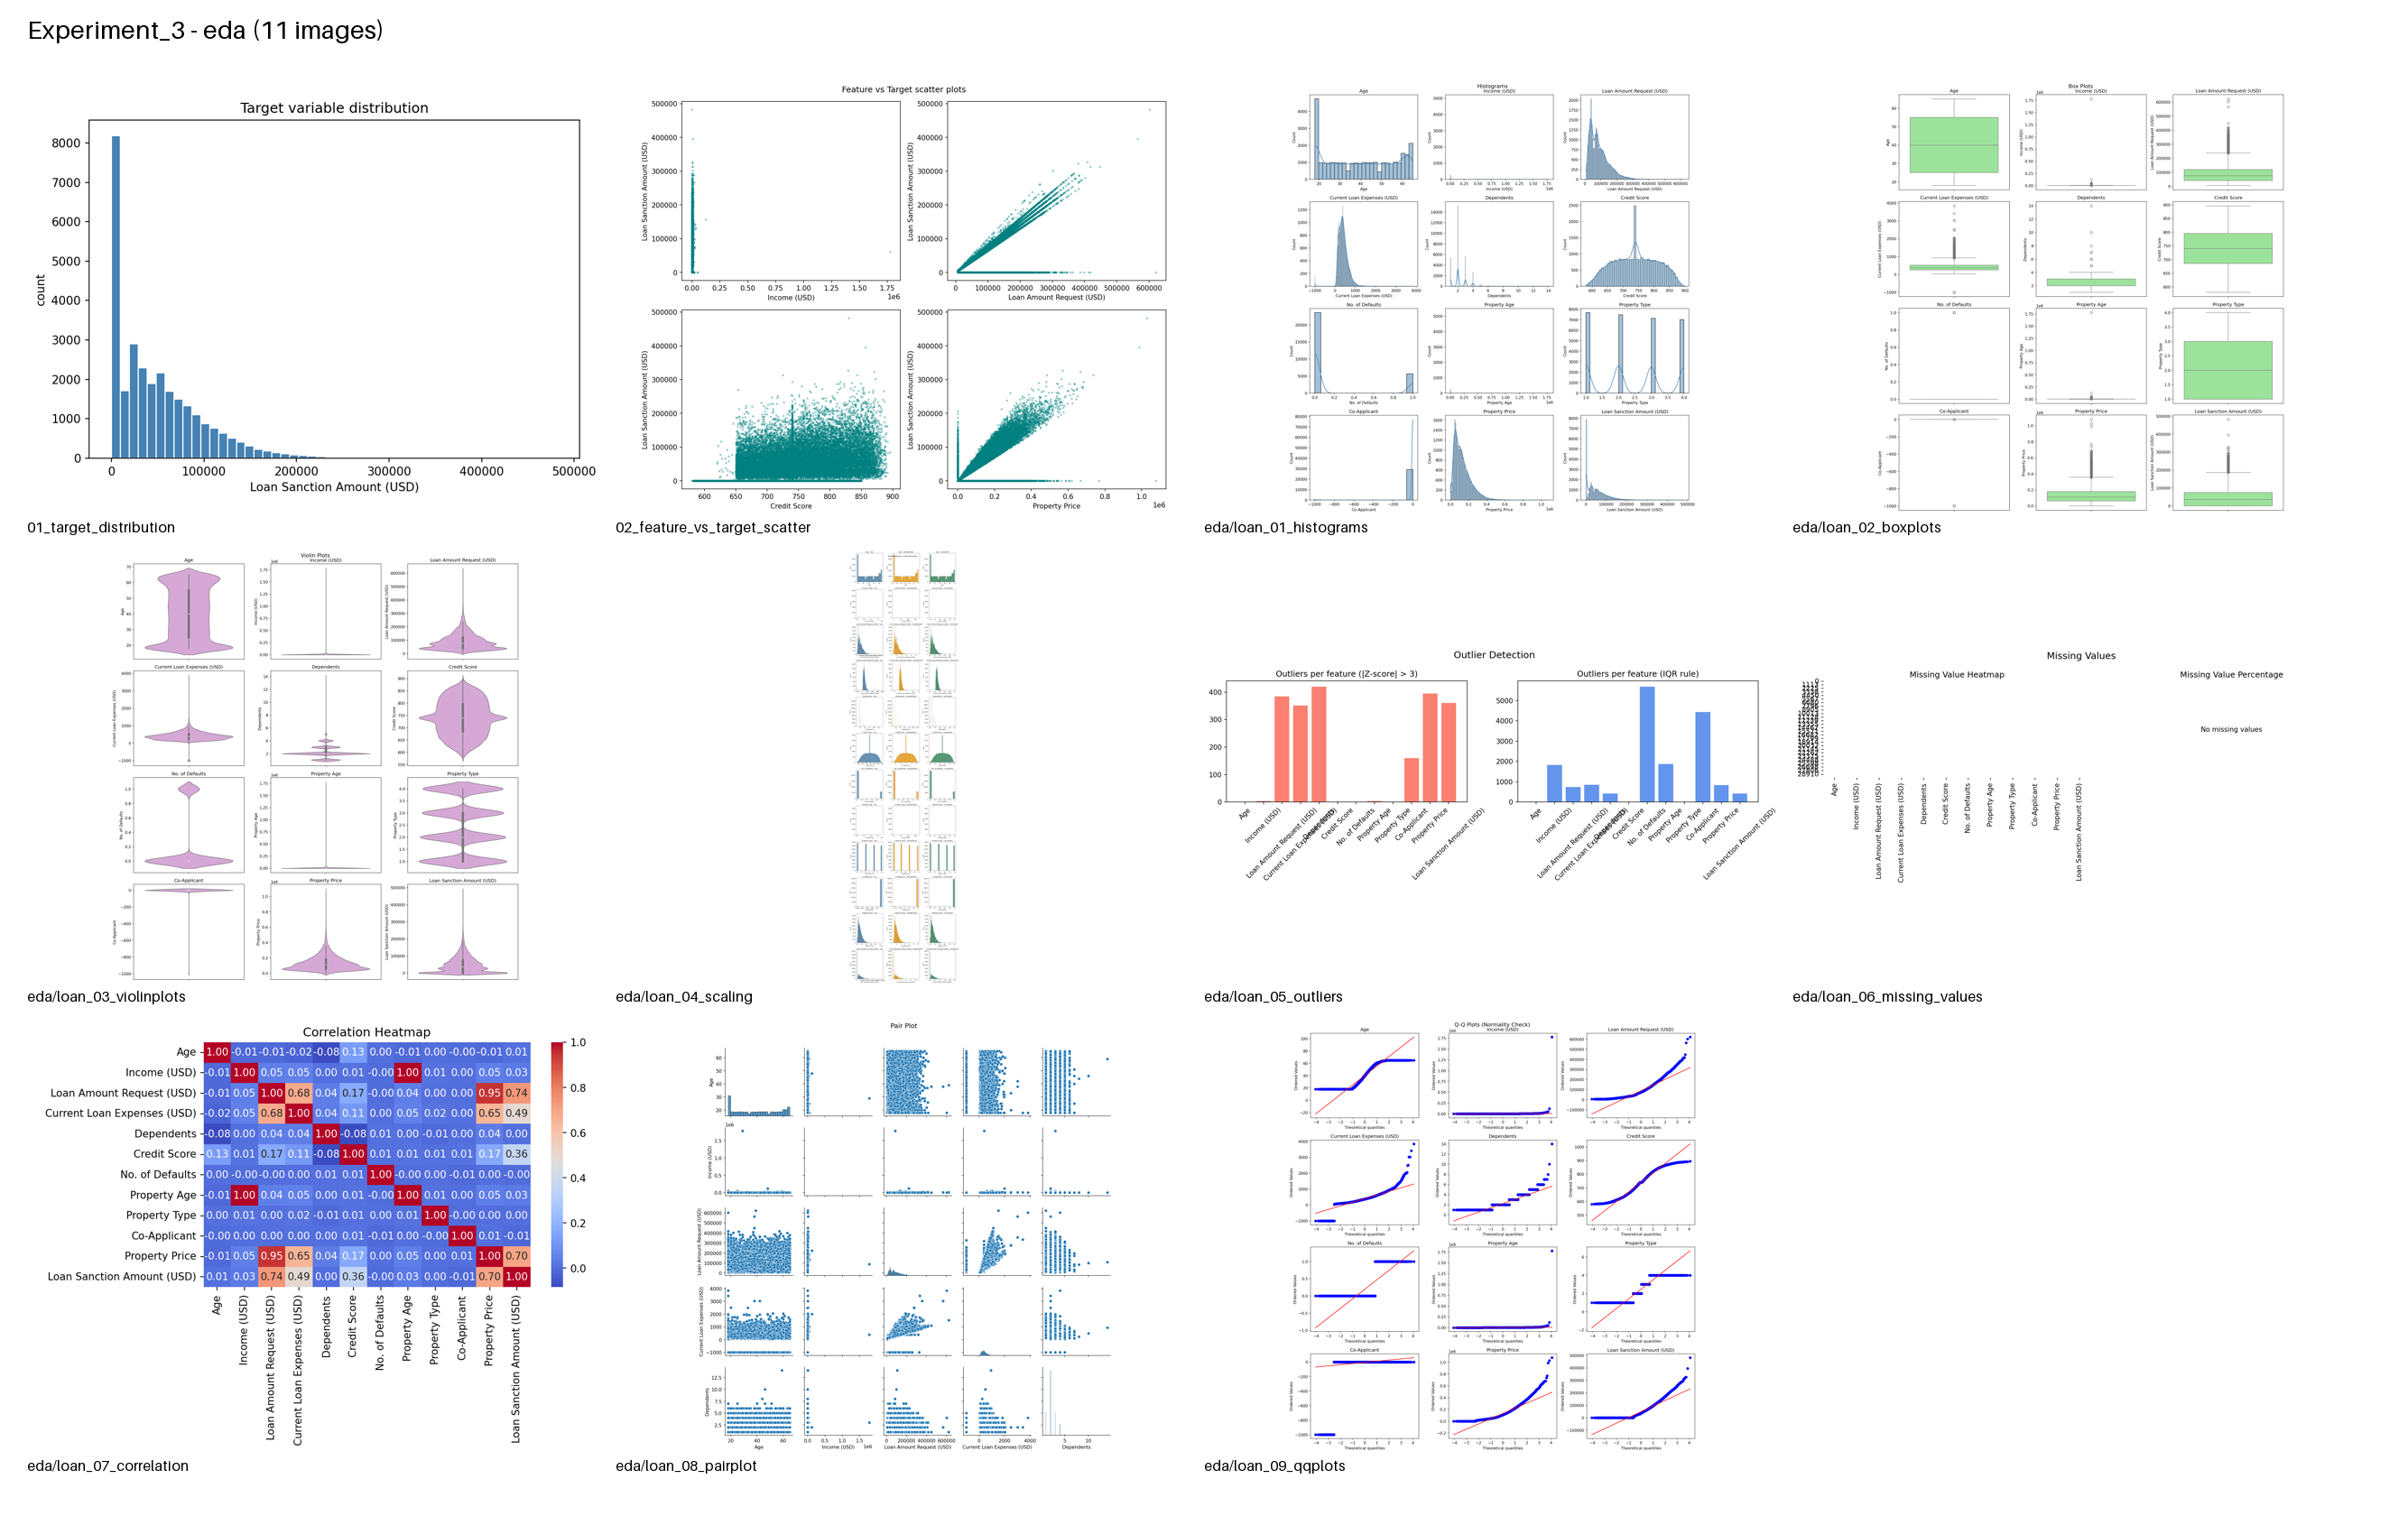
\includegraphics[width=0.95\linewidth]{outputs/Experiment_3_eda_combined.png}
\caption{Target distribution, feature vs target scatter plots, and the histogram, box plot, violin,
scaling, outlier, missing value, correlation, pair plot and Q-Q panels for the raw numeric features.}
\end{figure}

\textbf{Inference:}

Loan Amount Request turned out to have an almost linear relationship with the sanctioned amount, around
0.74 correlation, easily the strongest single predictor in the whole set. Income and Property Price
were far noisier by comparison, not much of a surprise. The missing value heatmap flags Type of
Employment, Property Age and Income as the real problem columns, and the box plots turned up a handful
of pretty extreme outliers in Property Price and Current Loan Expenses that were worth keeping an eye
on later.

\section{Data Preprocessing}
\begin{itemize}
\item Numeric columns filled with the median, categorical with the mode. Rows with an invalid target
just got dropped.
\item The 9 categorical columns were one-hot encoded, dropping the first category each time to avoid
the dummy trap.
\item All 45 features got standardized, which matters a lot here since Ridge, Lasso and Elastic Net
all penalize coefficient size directly.
\item Identifier columns (Customer ID, Name, Property ID) were dropped before modeling.
\end{itemize}

\begin{lstlisting}[caption={Grid search over Ridge, Lasso and Elastic Net, 5 fold CV}]
param_grids = {
    "Ridge": (Ridge(), {"alpha": [0.01, 0.1, 1, 10, 100]}),
    "Lasso": (Lasso(max_iter=50000), {"alpha": [0.001, 0.01, 0.1, 1, 10]}),
    "Elastic Net": (ElasticNet(max_iter=50000),
        {"alpha": [0.01, 0.1, 1, 10], "l1_ratio": [0.2, 0.5, 0.8]}),
}
for name, (model, grid) in param_grids.items():
    search = GridSearchCV(model, grid, cv=5, scoring="r2")
    search.fit(X_train_scaled, y_train)
\end{lstlisting}

\section{Machine Learning Algorithm}

\textbf{Linear Regression} fits $y = w^Tx + b$ by minimizing squared error, no penalty on the weights
at all.

\textbf{Ridge Regression} adds an L2 penalty, $\|y - Xw\|^2 + \alpha\|w\|_2^2$, which shrinks
coefficients toward zero but never quite lets them get there.

\textbf{Lasso Regression} uses an L1 penalty instead, $\|y - Xw\|^2 + \alpha\|w\|_1$, and this one can
actually push coefficients all the way to zero.

\textbf{Elastic Net} mixes both penalties together, aiming for a middle ground between Ridge's
stability and Lasso's sparsity, and it tends to handle correlated features a bit more gracefully than
pure Lasso does on its own.

\section{Experimental Setup}
\begin{tabular}{ll}
\toprule
Python Version & 3.11.9 \\
Scikit-Learn Version & 1.7.2 \\
IDE & Anaconda Navigator / VS Code \\
Operating System & Windows 11 \\
Hardware & \\
\bottomrule
\end{tabular}

\section{Hyperparameter Selection}
\begin{tabular}{ll}
\toprule
Parameter & Value\\
\midrule
Ridge alpha grid & 0.01, 0.1, 1, 10, 100 \\
Lasso alpha grid & 0.001, 0.01, 0.1, 1, 10 \\
Elastic Net grid & alpha in \{0.01,0.1,1,10\}, l1\_ratio in \{0.2,0.5,0.8\} \\
\bottomrule
\end{tabular}

\vspace{0.3cm}
\begin{tabular}{llll}
\toprule
Model & Search Method & Best Parameters & Best CV R2 \\
\midrule
Ridge & Grid Search & alpha = 100 & 0.5812 \\
Lasso & Grid Search & alpha = 10 & 0.5775 \\
Elastic Net & Grid Search & alpha = 0.1, l1\_ratio = 0.5 & 0.5904 \\
\bottomrule
\end{tabular}

\section{Results}

\textbf{Cross Validation Performance (K=5)}

{\small
\begin{tabular}{p{2.6cm}rrrr}
\toprule
Model & MAE & MSE & RMSE & R2 \\
\midrule
Linear Regression & 21122.68 & 9.69e8 & 31130.38 & 0.5857 \\
Ridge & 21140.84 & 9.62e8 & 31015.07 & 0.5888 \\
Lasso & 21113.68 & 9.65e8 & 31060.66 & 0.5876 \\
Elastic Net & 21325.89 & 9.57e8 & 30930.64 & 0.5911 \\
\bottomrule
\end{tabular}
}

\vspace{0.3cm}
\textbf{Test Set Performance}

{\small
\begin{tabular}{p{2.6cm}rrrr}
\toprule
Model & MAE & RMSE & R2 & Search Time (s) \\
\midrule
Linear Regression & 20760.58 & 29915.93 & 0.6021 & 0.05 \\
Ridge & 20782.62 & 29930.74 & 0.6017 & 10.8 \\
Lasso & 20751.62 & 29915.28 & 0.6021 & 692.4 \\
Elastic Net & 21035.64 & 30148.24 & 0.5959 & 22.9 \\
\bottomrule
\end{tabular}
}

Search time above is the full GridSearchCV run for that model, not a single fit, a few of the low-alpha
Lasso candidates just took forever to converge.

\vspace{0.3cm}
\textbf{Coefficient Comparison (three largest in the plain Linear model)}

{\small
\begin{tabular}{p{3cm}rrrr}
\toprule
Feature & Linear & Ridge & Lasso & Elastic Net \\
\midrule
Property Age & -46130.01 & -929.64 & -10.53 & -88.91 \\
Income (USD) & 46116.08 & 912.03 & 0.00 & 71.18 \\
Loan Amount Request & 34705.31 & 33215.74 & 34503.20 & 24888.48 \\
\bottomrule
\end{tabular}
}

\section{Result Visualization}

\begin{figure}[H]
\centering
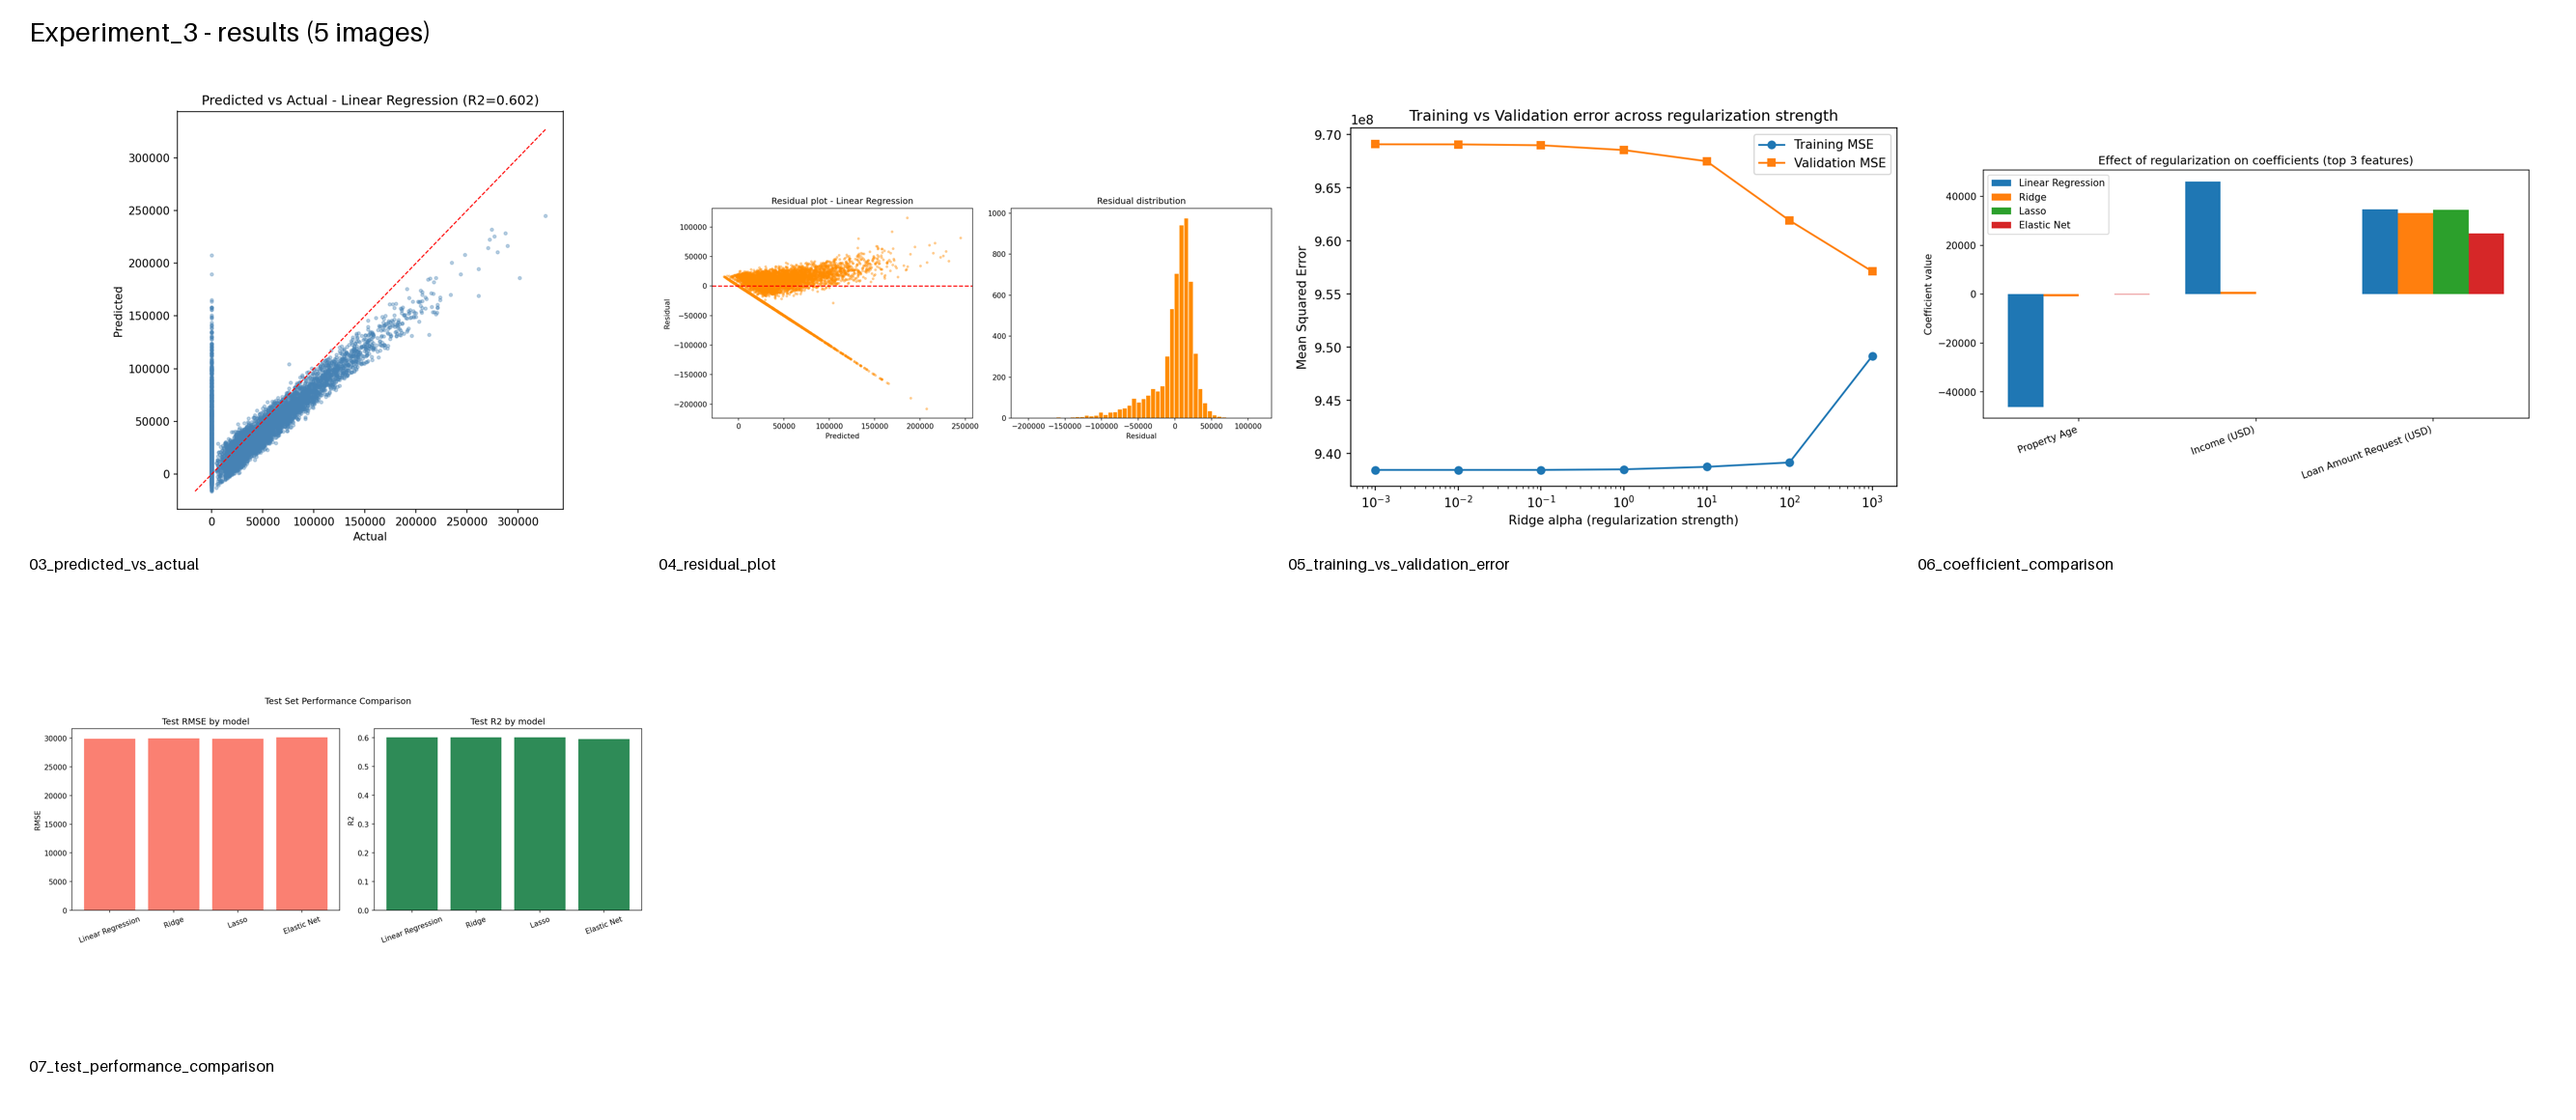
\includegraphics[width=0.95\linewidth]{outputs/Experiment_3_results_combined.png}
\caption{Predicted vs actual scatter, residual plot, training vs validation error across Ridge alpha,
coefficient comparison, and test set RMSE/R2 comparison across all four models.}
\end{figure}

\textbf{Inference:}

Predictions track the diagonal reasonably closely for small to mid loan amounts, but the model clearly
under-predicts the biggest ones, there is just less data up there to learn from. The residual plot has
a mild downward trend instead of a random scatter, so some non-linear structure is still slipping
through uncaptured. Training and validation MSE stay close together until around alpha=10 and then
climb together at high alpha, which is underfitting kicking in. The coefficient chart honestly tells
the best story in the whole report, Property Age and Income swing wildly under plain Linear Regression,
about 46 thousand in either direction, Ridge tames that down a lot, and Lasso all but erases it, while
Loan Amount Request just stays large and stable no matter which model you look at.

\section{Discussion}
Regularization did not really beat the plain Linear Regression baseline on accuracy, both land around
R2=0.60 on the test set. What it clearly did give back was more trustworthy coefficients, those wild
swings in Property Age and Income under plain Linear Regression look a lot like overfitting to
collinearity between the two, and Ridge and Lasso both settle that down nicely. Lasso zeroed out 5 of
the 45 coefficients, mostly one-hot columns that were not carrying much independent signal once the
strong numeric predictors were already in the model. The leftover residual pattern makes me think a
non-linear model would help more at this point than any further regularization tuning would.

\section{Conclusion}
Linear Regression is already sitting close to the practical ceiling for this feature set, test R2
around 0.60, and Ridge, Lasso and Elastic Net mostly earn their keep through steadier coefficients
rather than a real accuracy bump. Ridge alpha=100 and Lasso alpha=10 both came out as fairly strong
settings, which fits with there being genuine collinearity in the data worth damping down.

\section{Learning Outcomes}
\begin{itemize}
\item Learned that regularization does not always move accuracy much, here its real value was
stabilizing coefficients that were clearly overfitting under plain Linear Regression.
\item Got a much better feel for the practical difference between Ridge shrinking weights and Lasso
zeroing them out entirely.
\item Learned to read a training vs validation error curve as an actual picture of overfitting and
underfitting rather than just a textbook definition.
\item Noticed GridSearchCV time can balloon when a model has convergence trouble at certain
hyperparameter values, not only from how big the grid itself is.
\end{itemize}

\section{References}
\begin{enumerate}
\item Stephen Marsland, ``Machine Learning - An Algorithmic Perspective'', 2nd Edition, Chapman and
Hall/CRC Machine Learning and Pattern Recognition Series, 2015.
\item Ethem Alpaydin, ``Introduction to Machine Learning'', 3rd Edition, The MIT Press, 2014.
\end{enumerate}

\end{document}
